\chapter{Generated data}
\section{Uniform}
\begin{figure}[H]
\centering
\begin{subfigure}{.8\textwidth}
	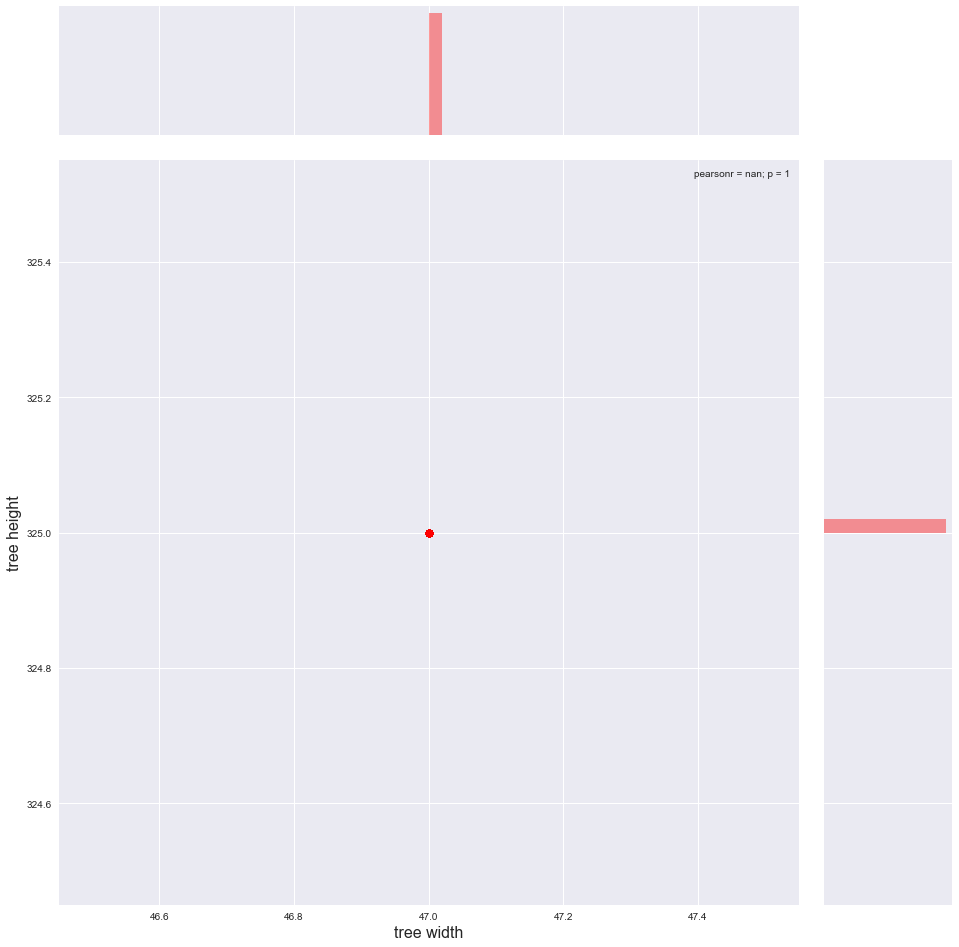
\includegraphics[width=.9\textwidth]{img/0_UNIFORM_plot.png}
\end{subfigure}%
\begin{subfigure}{.2\textwidth}
  \centering
  \begin{minipage}{1\textwidth}
\textbf{Widths:}
\
min: 47
\\
max: 47
\\
mean: 47.00
\\
variance: 0.00
\\
std: 0.00
\\
skewness: 0.00
\\
kurtosis: -3.00
\\\\
\textbf{Heights:}
\\
min: 109
\\
max: 109
\\
mean: 109.00
\\
variance: 0.00
\\
std: 0.00
\\
skewness: 0.00
\\
kurtosis: -3.00
  \end{minipage}
\end{subfigure}
\caption{Data distribution for 0\_Uniform.in}
\label{appendix:data:uniform}
\source{Compiled by the authors}
\end{figure}
\section{Random}
\begin{figure}[H]
\centering
\begin{subfigure}{.8\textwidth}
	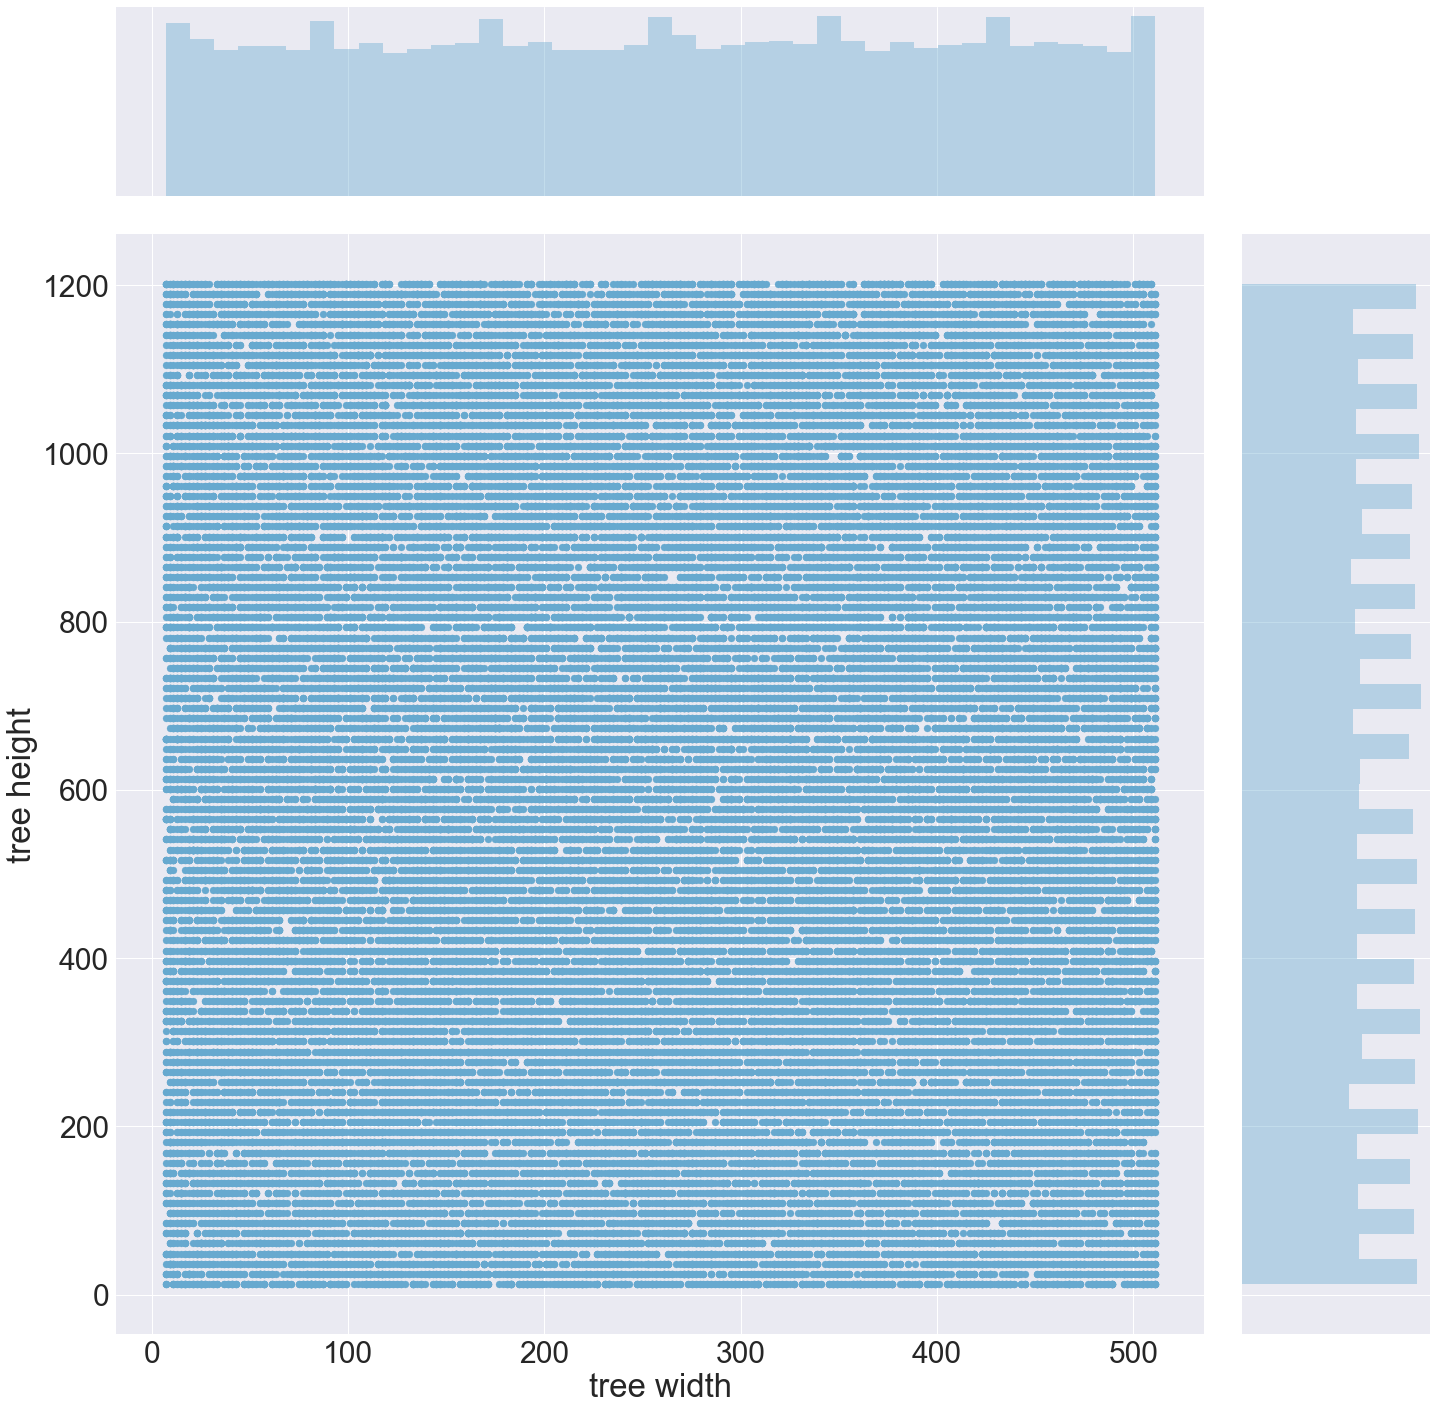
\includegraphics[width=.9\textwidth]{img/1_RAND_plot.png}
\end{subfigure}%
\begin{subfigure}{.2\textwidth}
  \centering
  \begin{minipage}{1\textwidth}
\textbf{Widths:}
\\
min: 7
\\
max: 511
\\
mean: 259.78
\\
variance: 21293.52
\\
std: 145.92
\\
skewness: -0.01
\\
kurtosis: -1.20
\\\\
\textbf{Heights:}
\\
min: 13
\\
max: 1201
\\
mean: 606.26
\\
variance: 120065.68
\\
std: 346.50
\\
skewness: 0.00
\\
kurtosis: -1.20
  \end{minipage}
\end{subfigure}
\caption{Data distribution for 1\_Rand.in}
\label{appendix:data:rand}
\source{Compiled by the authors}
\end{figure}

\section{Random with constant height}
\begin{figure}[H]
\centering
\begin{subfigure}{.8\textwidth}
	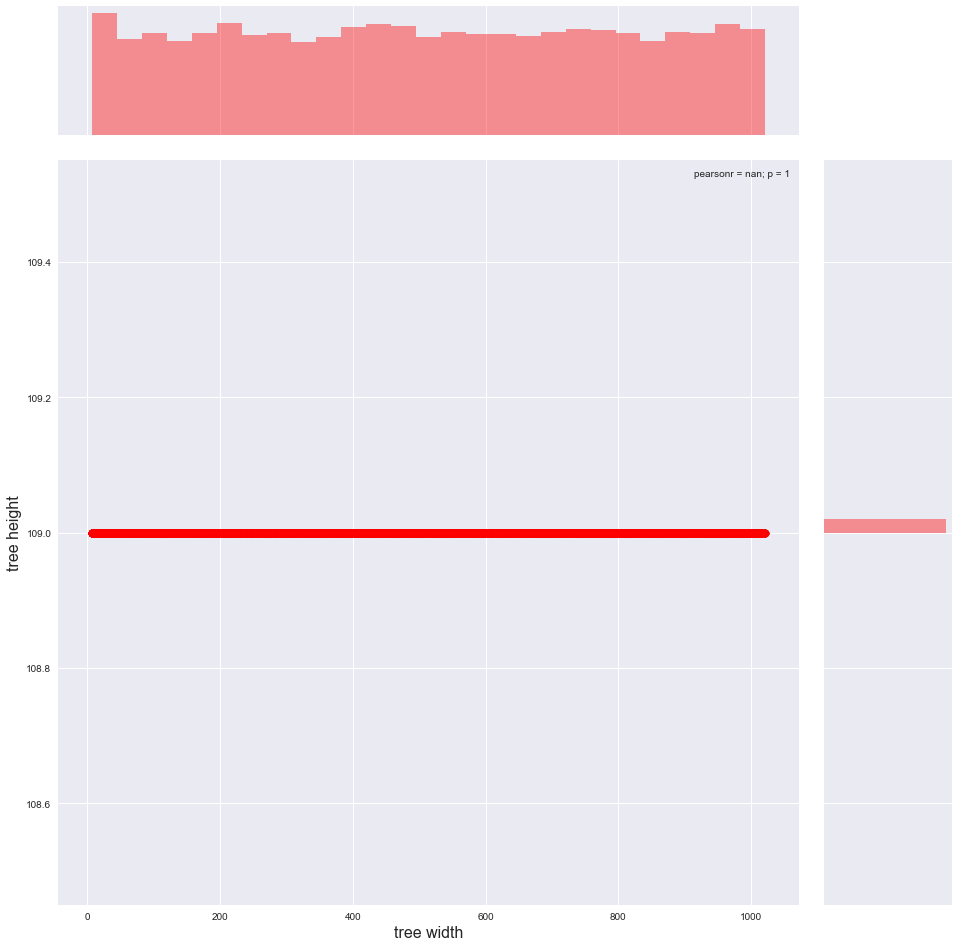
\includegraphics[width=.9\textwidth]{img/2_RANDCONSTHEIGHT_plot.png}
\end{subfigure}%
\begin{subfigure}{.2\textwidth}
  \centering
  \begin{minipage}{1\textwidth}
\textbf{Widths:}
\\
min: 7
\\
max: 511
\\
mean: 258.52
\\
variance: 21358.88
\\
std: 146.15
\\
skewness: -0.00
\\
kurtosis: -1.20
\\\\
\textbf{Heights:}
\\
min: 109
\\
max: 109
\\
mean: 109.00
\\
variance: 0.00
\\
std: 0.00
\\
skewness: 0.00
\\
kurtosis: -3.00
  \end{minipage}
\end{subfigure}
\caption{Data distribution for 2\_Randconstheight.in}
\label{appendix:data:randconstheight}
\source{Compiled by the authors}
\end{figure}
\section{Random with constant width}
\begin{figure}[H]
\centering
\begin{subfigure}{.8\textwidth}
	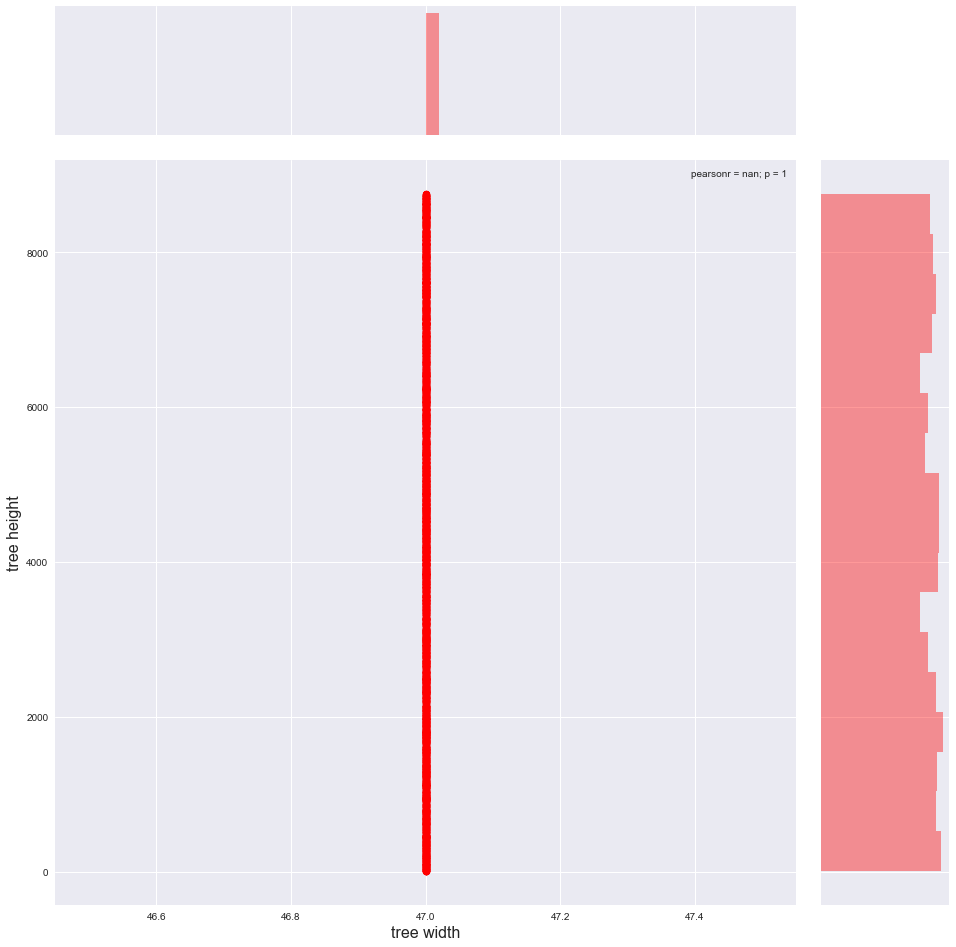
\includegraphics[width=.9\textwidth]{img/3_RANDCONSTWIDTH_plot.png}
\end{subfigure}%
\begin{subfigure}{.2\textwidth}
  \centering
  \begin{minipage}{1\textwidth}
\textbf{Widths:}
\\
min: 47
\\
max: 47
\\
mean: 47.00
\\
variance: 0.00
\\
std: 0.00
\\
skewness: 0.00
\\
kurtosis: -3.00
\\\\
\textbf{Heights:}
\\
min: 13
\\
max: 1201
\\
mean: 607.04
\\
variance: 119714.09
\\
std: 346.00
\\
skewness: -0.00
\\
kurtosis: -1.20
  \end{minipage}
\end{subfigure}
\caption{Data distribution for 3\_Randconstwidth.in}
\label{appendix:data:randconstwidth}
\source{Compiled by the authors}
\end{figure}
\section{Skewed}
\begin{figure}[H]
\centering
\begin{subfigure}{.8\textwidth}
	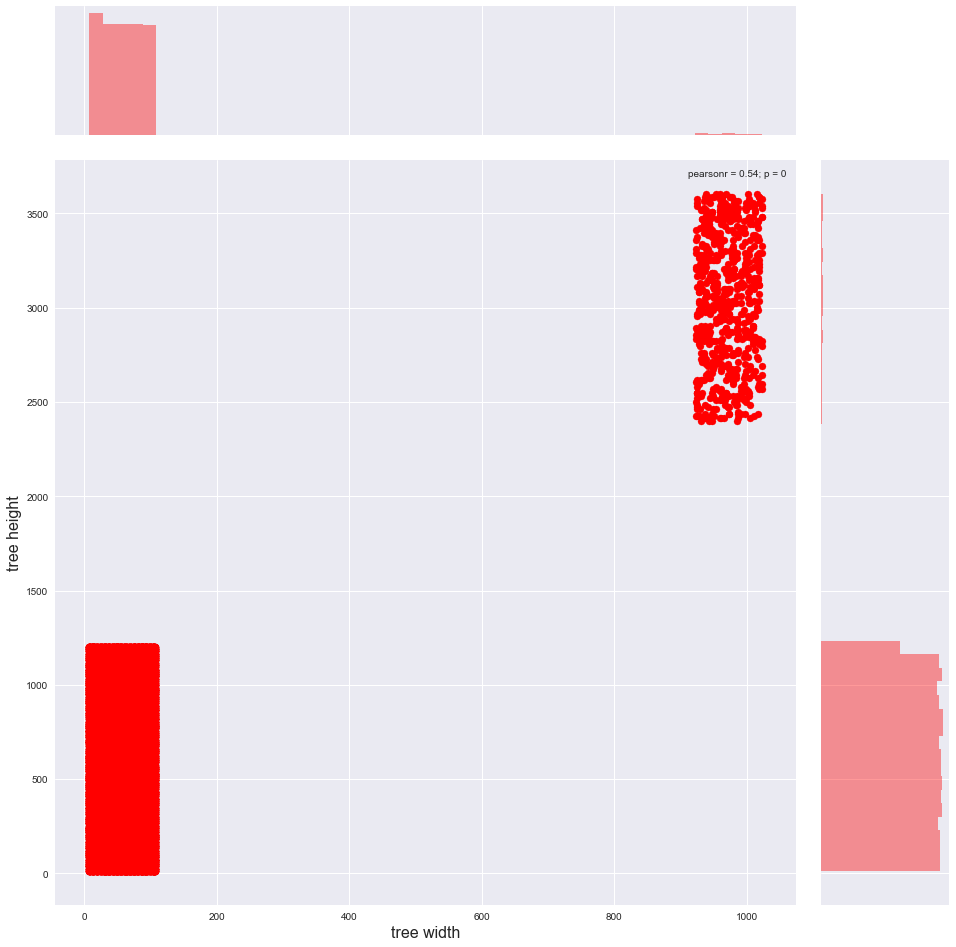
\includegraphics[width=.9\textwidth]{img/4_SKEWED_plot.png}
\end{subfigure}%
\begin{subfigure}{.2\textwidth}
  \centering
  \begin{minipage}{1\textwidth}
\textbf{Widths:}
\\
min: 7
\\
max: 511
\\
mean: 60.90
\\
variance: 2490.82
\\
std: 49.91
\\
skewness: 5.19
\\
kurtosis: 40.29
\\\\
\textbf{Heights:}
\\
min: 13
\\
max: 1201
\\
mean: 195.35
\\
variance: 17598.95
\\
std: 132.66
\\
skewness: 2.40
\\
kurtosis: 14.07
  \end{minipage}
\end{subfigure}
\caption{Data distribution for 4\_Skewed.in with 1\% total skewed options}
\label{appendix:data:skewed}
\source{Compiled by the authors}
\end{figure}
\section{Skewed with constant height}
\begin{figure}[H]
\centering
\begin{subfigure}{.8\textwidth}
	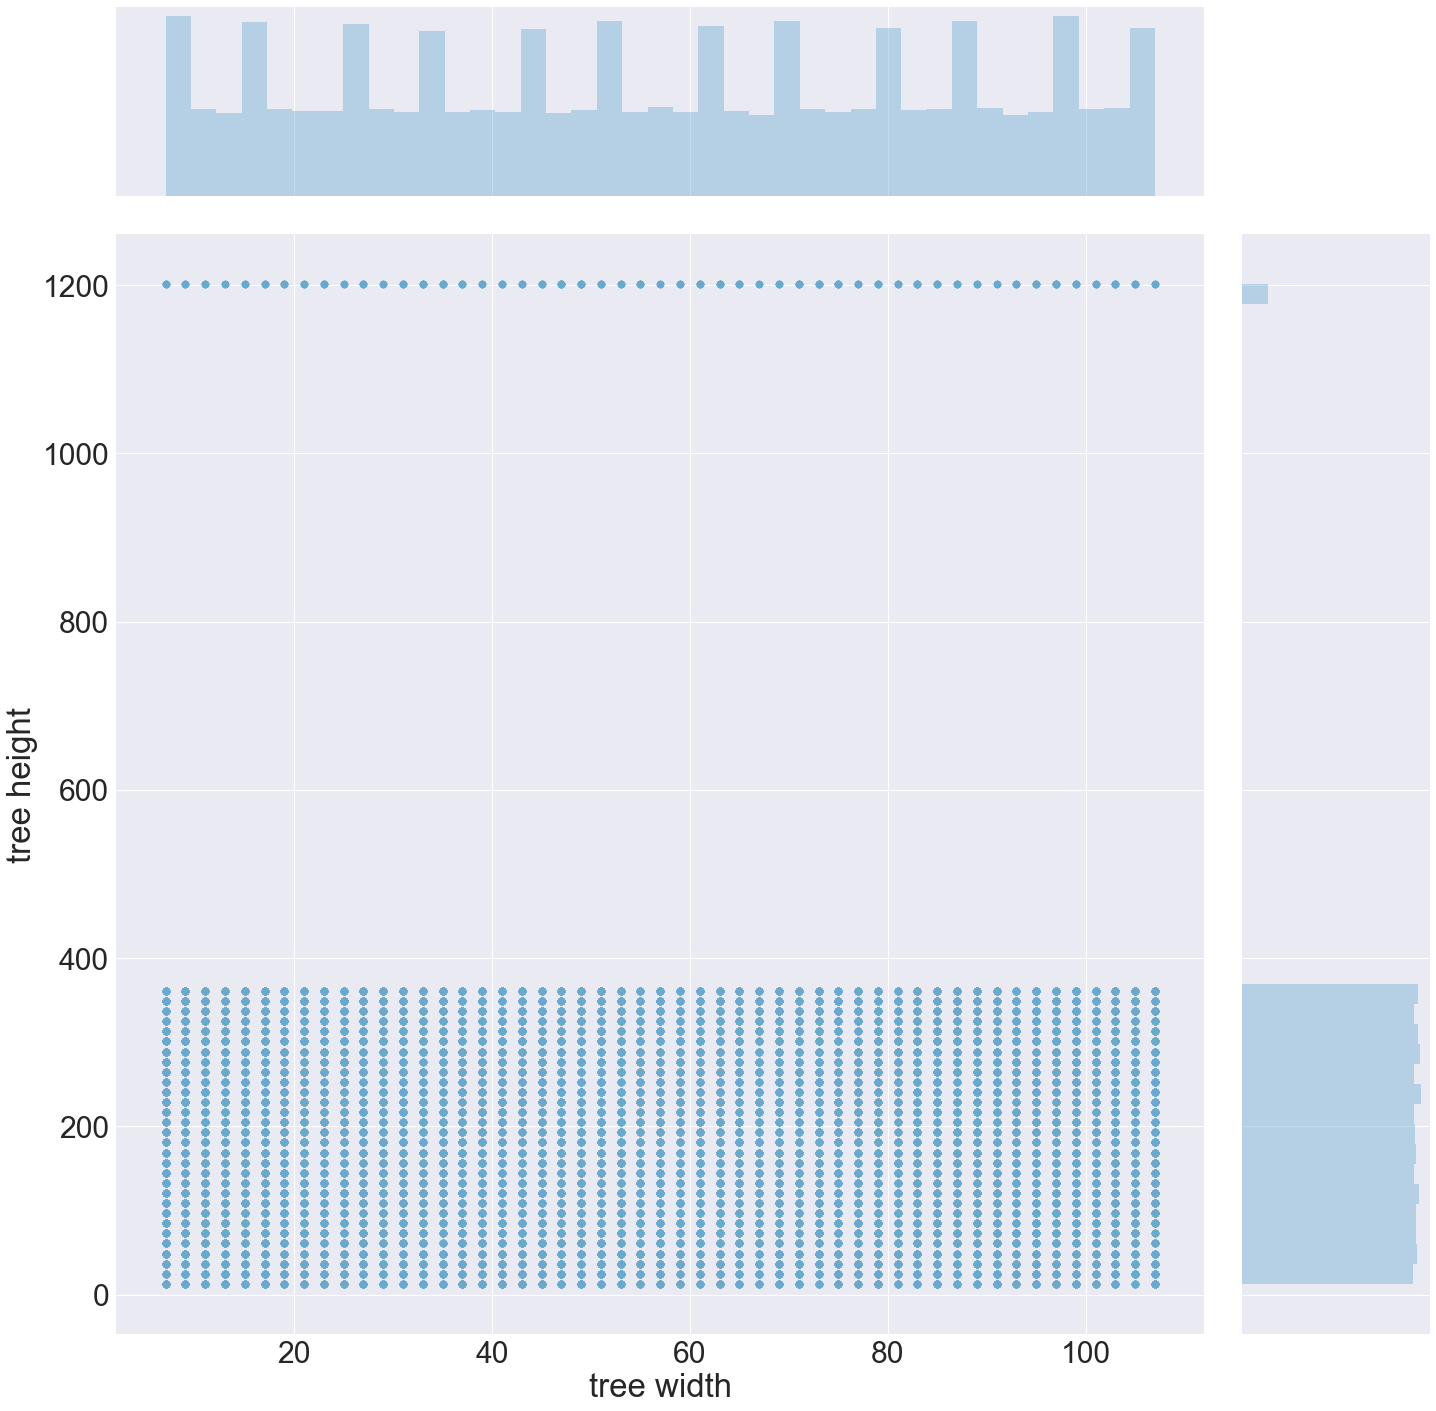
\includegraphics[width=.9\textwidth]{img/5_SKEWEDCONSTHEIGHT_plot.png}
\end{subfigure}%
\begin{subfigure}{.2\textwidth}
  \centering
  \begin{minipage}{1\textwidth}
\textbf{Widths:}
\\
min: 7
\\
max: 511
\\
mean: 61.06
\\
variance: 2493.88
\\
std: 49.94
\\
skewness: 5.15
\\
kurtosis: 39.87
\\\\
\textbf{Heights:}
\\
min: 13
\\
max: 1201
\\
mean: 602.58
\\
variance: 121471.29
\\
std: 348.53
\\
skewness: 0.01
\\
kurtosis: -1.22
  \end{minipage}
\end{subfigure}
\caption{Data distribution for 5\_Skewedconstheight.in with 1\% total skewed options}
\label{appendix:data:skewedconstheight}
\source{Compiled by the authors}
\end{figure}
\section{Skewed with constant width}
\begin{figure}[H]
\centering
\begin{subfigure}{.8\textwidth}
	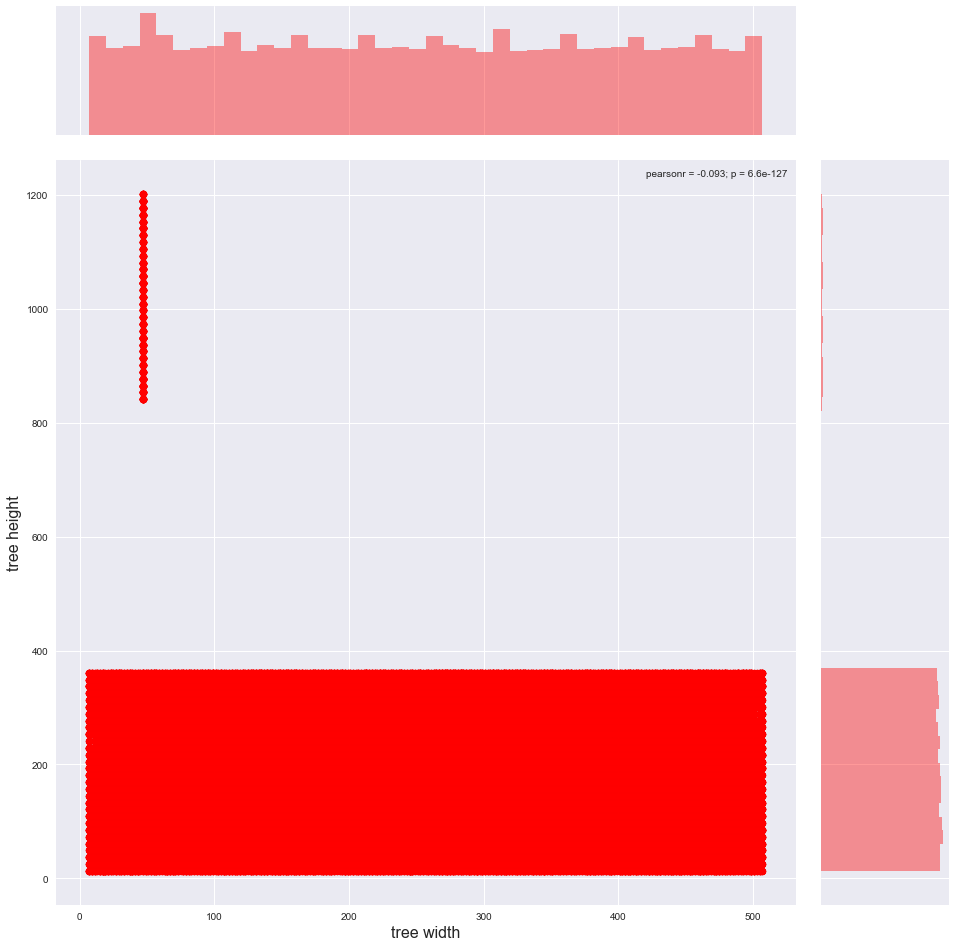
\includegraphics[width=.9\textwidth]{img/6_SKEWEDCONSTWIDTH_plot.png}
\end{subfigure}%
\begin{subfigure}{.2\textwidth}
  \centering
  \begin{minipage}{1\textwidth}
\textbf{Widths:}
\\
min: 7
\\
max: 507
\\
mean: 254.24
\\
variance: 21164.27
\\
std: 145.48
\\
skewness: 0.02
\\
kurtosis: -1.21
\\\\
\textbf{Heights:}
\\
min: 13
\\
max: 1201
\\
mean: 194.23
\\
variance: 17615.88
\\
std: 132.72
\\
skewness: 2.41
\\
kurtosis: 14.05
  \end{minipage}
\end{subfigure}
\caption{Data distribution for 6\_Skewedconstwidth.in with 1\% total skewed options}
\label{appendix:data:skewedconstwidth}
\source{Compiled by the authors}
\end{figure}